% A document built into a build folder (-B) whose path has a space
% (test/run.mjs builds it so). LaTeX, bibtex, and dvisvgm run in that
% folder, and \include writes the included file's .aux to a folder in it.
% A table of contents, a \ref each way, a \cite, a TikZ picture, and a
% term that the config marks.
\documentclass{article}
\usepackage{tikz}
\usepackage{hyperref}
\newcommand\term[1]{\emph{#1}}
\begin{document}
\tableofcontents
\section{Spaces}\label{sec:spaces}
A \term{space word}, the included part in section~\ref{sec:part}, and a
citation~\cite{spacebook}.
\begin{center}
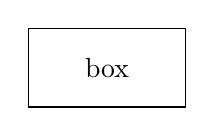
\begin{tikzpicture}
  \draw (0,0) rectangle (2,1);
  \node at (1,0.5) {box};
\end{tikzpicture}
\end{center}
\section{Included part}\label{sec:part}
Text of the included part, after section~\ref{sec:spaces}.

\bibliographystyle{plain}
\bibliography{test-builddirspace}
\end{document}
